\chapter{Detecção de fraude}

A fraude pode ter origem tanto interna quanto externa. Uma empresa está sujeita à fraude por seus administradores (denominada de alto-nível) ou empregados que não sejam gestores (baixo-nível) \cite{Phau2010}. Em um documento de 2012 \cite{ACFE2012}, a Associação de Investigadores de Fraude Certificados (Association of Certified Fraud Examiners, ACFE) definiu a fraude interna como ``a exploração ilegal dos recursos e bens de uma empresa, por um empregado, para enriquecimento próprio''\footnote{The use of one’s occupation for personal enrichment through the deliberate misuse or misapplication of the employing organization’s resources or assets.}.

Os autores da fraude externa dividem-se em três perfis: casual, criminal e crime organizado \cite{Phua2010}. Criminosos casuais apresentam comportamento aleatório, transgredindo as leis quando têm oportunidade, tentação ou em períodos de dificuldades financeiras. Por outro lado, indivíduos ou grupos organizados são mais perigosos porque tentam esconder ou dissimular sua verdadeira identidade, além de evoluir seu \emph{modus operandi} com o tempo, tentando burlar os sistemas de detecção e evitar a sua identificação. Assim, é importante levar-se em consideração essa constante interação entre os sistemas de detecção e os fraudadores profissionais. Essas categorias de fraudadores geralmente atuam em um setor específico: as fraudes internas e de seguro são mais frequentemente exploradas por criminosos comuns, enquanto fraudes de cartão de crédito e telecomunicações são vítimas de fraudadores profissionais.

O monitoramento de sistemas com o objetivo de encontrar comportamentos fraudulentos já existia muito antes da utilização de sistemas computacionais tornarem-se ferramentas comuns. Antes havia um processo denominado auditoria: gerar, armazenar e revisar um registro cronológico de eventos de um sistema \cite[p. 7]{Bace2000}. Os principais objetivos desses sistemas são identificar os usuários do sistema, impedir o uso impróprio, e auxiliar na reconstrução de eventos e na estimativa, quantificação e qualificação de danos.

O primeiro trabalho a considerar necessária a auditoria automática de sistemas foi \citet{Anderson1972}. Nesse trabalho, Anderson classifica os riscos e ameaças a sistemas, diferenciando fontes internas e externas, como na figura \ref{fig:and}. Também cita diversos objetivos para um sistema de auditoria:

\begin{itemize}
\item Prover informações suficientes para que o problema possa ser localizado, mas que não exponham detalhes que possibilitem um ataque.
\item Obter dados de diversas fontes para otimizar o conteúdo do banco de dados.
\item Discernir uma atividade ``normal'' do sistema, para que se possa detectar abusos interno.
\item Levar em consideração as estratégias dos invasores no projeto do sistema.
\end{itemize}

\begin{figure}[h!]
\centering
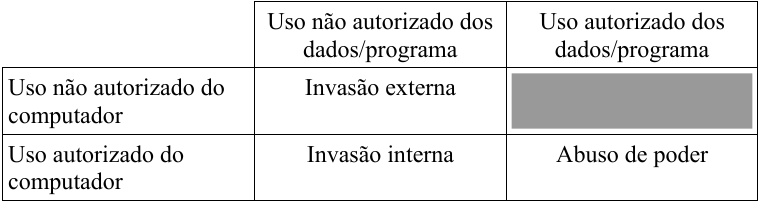
\includegraphics[width=0.75\textwidth]{img/anderson.png}
\caption{Matriz de ameaças}
\label{fig:and}
\end{figure}

A detecção de fraude é apenas uma das etapas de um sistema chamado de \emph{controle de fraude}. Nesse contexto, a detecção automática ajuda a reduzir o trabalho manual de verificação das instâncias. O objetivo principal desses sistemas é identificar padrões de transações suspeitas em meio às transações comuns de uma organização. O fraudador pode, por exemplo, contratar um seguro usando informações de outra pessoa ou informações falsas. O sistema procura detectar e impedir a fraude o mais cedo possível.

Geralmente não é possível ter absoluta certeza sobre a legitimidade das transações de um negócio a partir dos dados disponíveis. Não seria possível verificar todas as entidades com as quais uma empresa mantém relações, que em algumas empresas podem ser milhares. Assim, não existe uma técnica infalível para a detecção de fraudes. Isso não significa que elas não possam ser detectadas. A melhor alterantiva, na prática, é uma busca penosa por possíveis evidências de fraude nos dados disponíveis \cite{Phua2010}. Métodos matemáticos e estatísticos são utilizados para comparar um banco de dados de transações existentes com as novas, com o objetivo de encontrar evidências de possíveis fraudes. Mesmo assim, geralmente há um processo de análise e revisão caso a caso por um especialista.

Ainda, segundo a pesquisa apresentada no mesmo trabalho, o motor analítico desse tipo de sistema é composto de Sistemas Imunológicos Artificiais, inteligência artificial, auditoria, bancos de dados, computação distribuída e paralela, econometria, sistemas especialistas, lógica nebulosa, algoritmos genéticos, aprendizagem de máquina, redes neurais, reconhecimento de padrões, estatística, visualização, entre outros.

Dois conceitos relacionados à detecção em geral são falsos positivos e falsos negativos. Falsos positivos são instâncias erroneamente classificadas, por exemplo, uma transação comum que é classificada como fraudulenta. Falsos positivos são o oposto: uma transação fraudulenta que é classificada como comum. O número de falsos positivos aumenta o trabalho desnecessário na fase de revisão, enquanto os falsos negativos reduzem a eficácia da detecção. A redução dos falsos positivos é um dos objetivos principais de um sistema de detecção. Os falsos negativos, no entanto, são quase impossíveis de serem eliminados completamente, em qualquer sistema de detecção.

Mesmo um sistema capaz de reconhecer sinais de fraudes existentes não é suficiente para um ambiente real. Fraudadores tentam constantemente superar os sistemas de detecção, evoluindo o se \emph{modus operandi} com o tempo, novos métodos são criados, novos fraudadores entram em atividade. Um sistema que almeje deter o maior número possível deve ser constantemente atualizado para se adaptar às mudanças de um ambiente tão dinâmico.

Dependendo do domínio da organização, para que um sistema possa prever fraudes com antecedência suficiente para que elas sejam evitadas, deve monitorar constantemente as novas transações em andamento. Esse fator reduz a utilização de sistemas que necessitam de um longo tempo de treinamento ou de análise. O ideal seria que ele estivesse em constante execução, analisando as transações conforme elas ocorrem. Para aplicações grandes ou descentralizadas, pode ser muito difícil conseguir isso sem afetar a performance geral das transações.

Para cada domínio, tipos diferentes de fraude podem existir, e mais de um tipo pode ocorrer simultaneamente, sem uma ordem definida. 

\section{Dados}

Os atributos das instâncias em um banco de dados usado para detecção de fraude geralmente limitam-se a valores binários, numéricos, categóricos ou uma mistura desses três. Os atributos específicos usados geralmente são semelhantes. Aplicações de seguro utilizam o histórico do cliente: tempo de contrato, histórico e total de pagamentos, lucro anual valor médio depositado em conta bancária. Para fraudes de crédito, informações sobre as transações: valor, data, localização geográfica, conta de destino, tempo de conta. Fraudes em seguros de automóveis utilizam valores binários para atributos como acidente e tratamento hospitalar, além de dados do motorista, custo, tipo de ferimento.

O número de instâncias positivas nesse tipo de bases de dados é geralmente muito reduzido: as fraudes representam um percentual muito pequeno em relação ao número de transações legítimas de uma organização, geralmente menor do que 20\%. Métodos de detecção de fraude nunca são perfeitos: deve existir um mecanismo para lidar com as fraudes que não são identificadas a tempo de serem impedidas.

A obtenção de bancos de dados reais para teste é difícil, já que empresas e organizações, por razões legais e competitvas não disponibilizam informações desse tipo. Assim, é difícil encontrar bases de dados públicos para que os testes sejam realizados. Uma alternativa é a criação de um banco de dados artificial, inspirado em dados reais. A eficácia dessa técnica é limitada pela capacidade do criador do banco em prever o maior número de casos possíveis, o que geralmente é muito inferior à variedade das situações reais. Mesmo assim, essa técnica é comumente empregada na fase de concepção e teste, devido à dificuldade de obtenção de dados.

\section{Implementação}

A maioria dos sistemas de detecção de fraude opera usando listas negras (\emph{black-lists}) de dados (transações, contas, etc.), que são comparadas com as nova instâncias. Algumas utilizam regras fixas para a classificação. A figura \ref{fig:fraud-data} mostra a organização dos dados nesses sistemas. Uma parte do banco de dados é usada para o treinamento. Esses são os dados onde o sistema aprenderá os padrões e regras utilizados para a detecção. O restante das instâncias é usada para a avaliação do treinamento. Também é comum que haja bancos de dados distintos para o treinamento e avaliação.

\begin{figure}[h!]
\centering
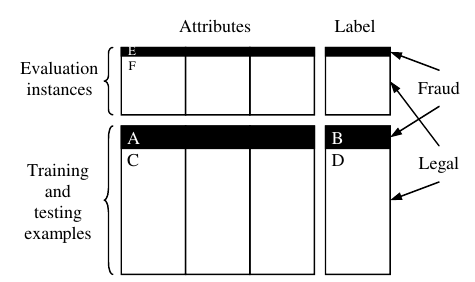
\includegraphics[width=0.75\textwidth]{img/fraud-data.png}
\caption{Dados para a análise}
\label{fig:fraud-data}
\end{figure}

A maioria dos estudos relacionados à detecção de fraude considera a detecção de \emph{outliers} como uma ferramenta principal de detecção \cite{Aral2011}. Existem muitos métodos aplicados à detecção de fraude: (1) auditoria, (2) sistemas especialistas, (3) lógica nebulosa (\emph{fuzzy}), (4) redes neurais, (5) reconhecimento de padrões, (6) árvores de decisão, (7) regressão, etc \cite{Huang2010}. As duas técnicas mais usadas são:

\begin{itemize}
\item Dados para treinamento classificadas (A + B + C + D) processados por um algoritmo supervisionado.
\item Instâncias legais (C) processadas por um algoritmo semi-supervisionado.
\end{itemize}

Algoritmos supervisionados examinam as instâncias previamente classificadas (A + B + C + D) para identificar matematicamente os padrões presentes nas classificadas como fraudulentas. Os algoritmos mais utilizados nessa categoria são as redes neurais. Outros algoritmos incluem máquinas de vetores de suporte (\emph{support vector machine}, SVM), árvores de decisão e raciocínio baseado em casos. Para aumentar a eficácia dos métodos supervisionados, esses algoritmos podem ser aplicados em sequência. Também podem ser combinados resultados de bancos de dados distintos.

Algoritmos não-supervisionados atuam sobre dados não classificados (A + C + E + F), e o seu objetivo é agrupar os dados em padrões, para que estes sejam mais facilmente analisados, combinando a detecção humana e a computação da máquina. Exemplos desses algoritmos são redes neurais não supervisionadas, análise de ligações (\emph{link analysis}) e mineração de grafos (\emph{graph mining}).

A combinação de algoritmos supervisionados (e de supervisionados e não-supervisionados), chamados de algoritmos híbridos, é uma grande área de pesquisa. Também são utilizados algoritmos supervisionados em bancos de dados que contêm apenas instâncias legais (C). Regras são geradas e testadas na base de dados, e aquelas que identificam padrões nesses dados são descartadas. Esses algoritmos são chamados de semi-supervisionados, porque, apesar de não fazerem distinção entre dados legais e ilegais, os dados ainda necessitam ser classificados para que sejam utilizados no seu treinamento.

\citet{Phua2010} fazem muitas críticas ao uso de dados previamente classificados para o treinamento dos sistemas. A classificação atrasa o processo de detecção, aumenta o tempo de reação a novos tipos de fraudes e pode ser cara e difícil de se obter. Pode ainda ser incorreta, tendenciosa e expor dados sigilosos, dependendo do tipo de aplicação. Assim, instâncias de treinamento e avaliação (A + C + E + F, sem classificações) devem ser combinadas e processadas por um algoritmo não-supervisionado, detectando regras, pontuações ou anomalias visuais nos dados avaliados.

\section{Granularidade}

Um sistema que detecte e reporte uma fraude muito tempo depois de ela ter ocorrido permite que o fraudador consiga causar um dano substancial. Em geral, esse tempo de resposta de um sistema a partir do momento em que uma fraude é concretizada até a sua detecção é crucial para a eficácia do sistema em de fato proteger o ambiente em que é inserido.

Os sistemas de detecção podem ser divididos em dois tipos gerais, denominados \emph{on-line} e \emph{off-line}, enquanto alguns incorporam características dos dois modelos e outros têm um processo distinto para ambos, que interagem entre si para gerar o resultado final \cite{Huang2010}.

\section{Critérios de avaliação}

A maioria dos departamentos que atuam na área de detecção de fraude utiliza valores monetários como medida de avaliação dos sistemas \cite{Phua2010}.

\citet{Phua2010} lista as diversas medidas de performance utilizadas em trabalhos recentes na área de detecção de fraude. Os métodos tradicionais de medição, como a taxa de positivos (número de fraudes detectadas corretamente dividido pelo número de fraudes verdadeiras) e a precisão a um determinado limite (número de instâncias classificadas corretamente, dividido pelo número total de instâncias) foram abandonados pelos trabalhos recentes, devido à natureza peculiar da detecção de fraude.

A razão para isso é que o custo das classificações errôneas, no caso da detecção de fraude, são irregulares, incertos, variam de exemplo a exemplo e podem variar conforme o tempo. Falsos negativos são geralmente mais custos do que falsos positivos. Um falso positivo geralmente leva apenas a uma verificação a mais por um especialista, infrutífera. Um falso negativo, no entanto, acarreta em uma fraude que não é detectada pelo sistema e não será reportada, deixando o fraudador impune.

Classificadores binários são aqueles que, para um dado conjunto de valores de entrada, geram como valor de saída um valor Booleano: verdadeiro ou falso, positivo ou negativo. Os sistemas de detecção de fraude se situam, na maioria dos casos, nessa categoria: os dados referentes a uma instância passam pelo sistema de detecção e são classificados como legítimos ou fraudulentos \cite{Bewick2004}. Sistemas mais complexos podem gerar saídas com mais informações sobre a instância, como o grau de certeza da previsão ou o grau de semelhança entre a instância e os dados da base.

A avaliação dos classificadores binários é feita com base em uma \emph{tabela de confusão}, conforme mostrado na tabela \ref{fraud:confusion}. Nessa tabela são listados o número de valores (ou porcentagem) para cada combinação de saída do sistema e a classificação real. Instâncias corretamente classificadas ocupam as colunas Positivo e Negativo, enquanto instâncias cujo classificação difere da realidade ocupam as colunas Falsos Positivos e Falsos Negativos.

\renewcommand{\arraystretch}{1.5}
\begin{table}[h!]
    \centering
    \begin{tabular}{c l c c}
        & & \multicolumn{2}{c}{\textbf{Dados reais}} \\
        \multirow{3}{5mm}{\begin{sideways}\parbox{20mm}{\textbf{Saída}}\end{sideways}} & \multicolumn{1}{c|}{} & Positivo & Negativo \\
        \cline{2-4}
        & \multicolumn{1}{c|}{Positivo} & Positivo & Falso positivo\\
        & \multicolumn{1}{c|}{Negativo} & Falso negativo & Negativo\\
    \end{tabular}
    \caption{Tabela de confusão}
    \label{fraud:confusion}
\end{table}

Como exemplo, inspirado em \citet{Bewick2004}, será apresentado um sistema de detecção de fraude de empréstimos simples, que considera como único atributo das instâncias o número de ocorrências de inadimplência. Nesse ambiente simplificado, a instância é considerada fraudulenta caso um limiar de ocorrências seja ultrapassado. Um exemplo de teste é mostrado na tabela \ref{fraud:ex}. A partir desses dados, a avaliação dos resultados é feita usando dois conceitos: sensitividade e especificidade.

\renewcommand{\arraystretch}{1.5}
\begin{table}[h!]
    \centering
    \begin{tabular}{c l c c c}
        & & \multicolumn{2}{c}{\textbf{Dados reais}} \\
        \multirow{3}{5mm}{\begin{sideways}\parbox{20mm}{\textbf{Saída}}\end{sideways}} & \multicolumn{1}{c|}{} & Fraude & Legítimo & \multicolumn{1}{|c}{Total} \\
        \cline{2-5}
        & \multicolumn{1}{c|}{Fraude}   & 300 & 200   & \multicolumn{1}{|c}{500}  \\
        & \multicolumn{1}{c|}{Legítimo} & 100 & 1000  & \multicolumn{1}{|c}{1100} \\
        \cline{2-5}
        & \multicolumn{1}{c|}{Total}    & 400 & 1200  & \multicolumn{1}{|c}{1600} \\
    \end{tabular}
    \caption{Tabela de confusão}
    \label{fraud:confusion}
\end{table}

\subsection{Sensibilidade e especificidade}

\emph{Sensitividade} refere-se à proporção de instâncias corretamente classificadas como positivas. \emph{Especificidade} refere-se à proporção de instâncias corretamente classificadas como negativas. No exemplo, a sensitividade é igual a 300 / 400 = 0.75; e a especificidade é igual a 1000 / 1200 = 0.8333. Ou, visto de outra maneira, 75\% das fraudes foram realmente classificadas como fraudes; e 83.33\% das instâncias legítimas foram classificadas como legítimas.

Apenas a consideração desses dois valores pode levar a uma correta avaliação dos resultados do teste, principalmente nos domínios da detecção de fraude. Uma alta sensitividade não necessariamente implica em uma alta especificidade, e vice versa. Dessas duas informações são derivados os \emph{valores preditivos positivos e negativos}.

\subsection{Valores preditivos}

O \emph{valor preditivo positivo} é a chance de uma instância ser realmente uma fraude caso seja classificada como tal pelo sistema. O \emph{valor preditivo negativo} é a chance de uma instância ser realmente legítima caso seja classificada como tal pelo sistema. Para os dados de exemplo, o valor preditivo positivo é 300 / 500 = 0.6; e o valor preditivo negativo é 1000 / 1100 = 0.9091. Ou, visto de outra maneira, 60\% das instâncias que foram classificadas como fraude eram realmente fraudes, e 90.91\% das instâncias classificadas como legítimas eram realmente legítimas.

Esses dois valores são o oposto da sensibilidade e especificidade, respectivamente. Enquanto os valores preditivos dão uma avaliação direta sobre os resultados dos testes, a sensibilidade e especificidade não são afetadas pela proporção dos valores nas instâncias. Uma alteração na proporção de fraudes alteraria aqueles, mas não estes.

\subsection{Taxas de verosimilhança}

A sensibilidade e especificidade tornam-se ainda mais úteis quando combinadas, gerando as taxas de verossimilhança. A taxa de verossimilhança de um resultado positivo (LR\textsuperscript{+}) é a razão entre a probabilidade de um resultado positivo no teste se a instância é realmente positiva (coluna "positivo" da tabela de confusão) e a probabilidade de um resultado positivo no teste se a instância é na verdade negativa:

\begin{equation}
    LR^{+}=\frac{sensitividade}{1 - especificidade}
\end{equation}

No exemplo, LR\textsuperscript{+} = 0.75 / (1 - 0.8333) = 4.4991. Isso significa que um resultado positivo nos testes é 4.4991 vezes mais provável para instâncias que são realmente positivas do que para aquelas que não são.

De maneira, similar, a taxa de verossimilhança negativa (LR\textsuperscript{-}) é a razão entre a probabilidade de um resultado negativo no teste se a instância é realmente negativa (coluna "negativo" da tabela de confusão) e a probabilidade de um resultado negativo no teste se a instância é na verdade positiva:

\begin{equation}
    LR^{-}=\frac{1 - sensitividade}{especificidade}
\end{equation}

No exemplo, LR\textsuperscript{-} = (1 - 0.75) / 0.8333 = 0.3, o que significa que um resultado negativo no teste é 0.3 vezes mais provável para instâncias que são realmente negativas do que para aquelas que não são.

Desses valores, pode-se atestar a utilidade do método para classificação. Uma alta taxa de verossimilhança positiva indica que o teste é útil para verificar se uma instância é positiva, enquanto uma alta taxa de verossimilhança negativa é útil para verificar se uma instância é negativa. Assim como os valores preditivos, essas taxas são sensíveis à predisposição dos dados na base de dados.

\subsection{Índice de Youden e ROC}

Os dados de teste do exemplo até agora consideraram apenas um valor como limiar de classificação. No entanto, em sistemas reais, é comum que sejam testados diversos valores para esse limiar sobre uma mesma base de dados, para que o melhor seja identificado e usado no sistema final. A tabela \ref{fraud:youden} é um exemplo de resultados para esse tipo de teste.

\begin{table}[h!]
    \centering
    \begin{tabular}{l c c c c c}
        \hline
        Limiar & Fraudes & Legítimos & Sensibilidade & Especificidade & Índice de Youden \\
        \hline
        0     & 400 &    0 & 1      & 0      & 0      \\
        1     & 395 &  400 & 0.9875 & 0.3333 & 0.3208  \\
        2     & 380 &  600 & 0.95   & 0.5    & 0.45   \\
        3     & 375 &  900 & 0.9375 & 0.75   & 0.6875 \\
        4     & 200 & 1000 & 0.5    & 0.8333 & 0.3333 \\
        99    &   0 & 1200 & 0      & 0      & 0      \\
        \hline
        Total & 400 & 1200 &        &        &        \\
        \hline
    \end{tabular}
    \caption{Exemplo de resultados para testes comparativos de limiares (inspirado em \citet{Bewick2004}}
    \label{fraud:youden}
\end{table}

Uma medida para a avaliação dos diferentes limiares pode ser a sensibilidade e especificidade. O índice de Youden é uma medida apropriada nesses casos (eq. \ref{fraud:yindex}). Esse índice é um valor normalizado na faixa [0, 1], onde 1 significa um teste perfeito, classificando todas as instâncias corretamente; e 0 significa um teste sem valor nenhum. A tabela \ref{fraud:yindex} mostra os valores para os resultados com diversos limiares. É importante notar como valores extremos maximizam a sensibilidade e a especificidade, mas apenas aqueles limiares que maximizam os dois valores recebem índices significativos.

\begin{equation}
    J = sensibilidade + especificidade - 1
    \label{fraud:yindex}
\end{equation}

Uma característica importante do índice de Youden é que ele estabelece uma equivalência na relevância dos falsos positivos e negativos. Quando um é mais relevante que o outro, devido à peculiaridades nos dados ou no domínio do problema, ele não é apropriado. Nesses casos, pode-se atribuir pesos diferentes a ambos os valores. Um exemplo de adaptação do cálculo do índice de Youden é mostrado abaixo. Nessa fórmula, os valores ainda são mantidos na mesma faixa, mas falsos positivos recebem o dobro da significância.

\begin{equation}
    J = 0.75 * sensibilidade + 0.25 * especificidade
\end{equation}

\iffalse

Uma alternativa é atribuir uma pontuação a cada instância de acordo com uma razão entre a similaridade com casos conhecidos de fraude e a dissimilaridade com casos legais.

\citet{Aral2011} utilizam o número de falsos positivos, falsos negativos e verdadeiros positivos como medida de performance do seu sistema.

\fi

\section{Trabalhos relacionados}

O sistema detecção de fraude no comércio eletrônico apresentado em \citet{Huang2010} é um exemplo de sistema que combina dois dois processos de diferentes granularidades que interagem entre si.

\citet{Aral2011} apresentam um sistema de detecção de fraude em prescrições médicas que calcula um fator de risco associado a cada prescrição. Matrizes de incidências são geradas através de uma medida de distância entre valores cruzados (\emph{cross-features}) de uma base de conhecimento. Dessas matrizes são geradas matrizes de riscos, e cada instância da base de dados cujo risco for maior que um limiar é relatada como uma possível fraude. Os autores indicam que o raciocínio por trás desse modelo é de que os padrões no comportamento fraudulento são \emph{outliers} quando considerados no contexto do \emph{dataset} como um todo. Os limiares são configuráveis, permitindo ao usuário um controle sobre o número de falsos positivos gerados.
